\documentclass[12pt, a4paper]{article}
\usepackage[utf8]{inputenc}
\usepackage[T1]{fontenc}
\usepackage{amsmath}
\usepackage{amssymb}
\usepackage{amsthm}
\usepackage{geometry}
\usepackage{color}
\usepackage{listings}
\usepackage[hidelinks]{hyperref}
\usepackage[dvipsnames]{xcolor}
\usepackage[polish]{babel}
\usepackage{graphicx}
\usepackage{subcaption}
\usepackage{float}

\geometry{
 a4paper,
 margin=1in,
}

\title{Sprawozdanie z Implementacji Algorytmu Jarvisa i Grahama}
\author{Artur Radwański - grupa 4}
\date{14 grudnia 2025}

\begin{document}

\maketitle

\section{Realizacja Ćwiczenia}
\subsection{Cel Ćwiczenia}
Celem ćwiczenia było zapoznanie się z algorytmami zamiatania wyznaczającymi otoczkę wypukłą, wraz z ich implementacją oraz
porównanie działania algorytmów na różnych zbiorach oraz z różnymi parametrami.

\subsection{Wstęp teoretyczny}
\paragraph{Otoczka wypukła} - dla dowolnego zbioru puntków S zawierającego co najmniej jeden element, to najmniejszy zbiór wypukły
zawierający w całości S. Jest ona uproszczeniem kształtu obiektu i znajduje zastosowanie w optymalizacji wykrywania kolizji i 
planowania ruchu.


\paragraph{Algorytm Grahama} - znajduje otoczkę wypukłą zaczynając od znalezienie wierzchołka skrajnego, który na pewno należy do
otoczki wypukłej (tutaj - punkt o najmniejszej współrzędnej y, a w przypadku remisu o najmniejszej współrzędnej x). Sortuje kątowo
wszystkie inne punkty względem tego pierwszego i tworzy stos na którym przechowuje kandydatów na wierzchołki otoczki wypukłej.
Algorytm gwarantuje, że po jego wykonaniu na stosie znajdują się tylko wierzchołki tworzące otoczkę wypukłą, w kolejności przeciwnej
do ruchu wskazówek zegara. Jego złożoność obliczeniowa to $O(n\log{n})$ - gdzie $n$ to liczba wierczhołków.

\noindent
Lista kroków:
\begin{enumerate}
    \item Znajdź punkt $p_{0}$ o najmniejszej współrzędnej y (najmniejszej współrzędnej x w przypadku remisu)
    \item Posortuj wszystkie pozostałe punkty, ze względu na kąt jaki odcinek $(p_{0},p)$ tworzy z dodatnim kierunkiem osi x.
    W przypadku remisu, zostw ten najbardziej oddalony.
    \item Uwtórz pusty stos. Włóż do niego punkty $p_{0},p_{1},p_{2}$, gdzie $p_{n}$ to $n$-ty punkt w posortowanej strukturze.
    \item Iteruj po kolejnych punktach, jeśli $p_{n}$ leży na lewo od ostatniego odcinka dodanego do otoczki, to dodaj 
    go na szczyt stosu i zacznij przetwarzać następny wierzchołek. Jeżeli $p_{n}$ leży na prawo od ostatniego odcinka dodanego do 
    otoczki, to zdejmij element ze szczytu stosu.
\end{enumerate}

\paragraph{Algorytm Jarvisa} - (pakowanie prezentu) Podobnie jak algorytm Grahama zaczyna od wybrania skrajnego punktu który na pewno
należy do otoczki wypukłej. Potem oblicza otoczkę, poprzez znajdywanie punktu tworzącego najmniejszy 
kąt zewnętrzy razem z ostatnim odcinkiem otoczki. Złożoność obliczeniowa to $O(nk)$ , gdzie $n$ to ilość punktów w zbiorze, a $k$ to
ilość wierzchołków w otoczce. Jeśli nie przyjmiemy żadnych założeń co do zbioru punktu, to złożoność sprowadza się do $O(n^{2})$

\noindent
Lista kroków:
\begin{enumerate}
    \item Znajdź punkt $p_{0}$ o najmniejszej współrzędnej y (w przypadku remisu o najmniejszej współrzędnej x).
    \item Każdy następny punkt $p_{i}$ to punkt który tworzy najmniejszy kąt zewnętrzny z ostatnim odcinkiem w otoczce (dla $p_{1}$ to
    najmniejszy kąt między $(p_{0},p_{1})$ a dodatnim kierunkiem osi x).
    \item Jeśli następny $p_{i}$ to $p_{0}$ to zakończ działanie algorytmu. Otoczka wypukła jest kompletna.
\end{enumerate}

\subsection{Szczegóły implementacji}
\paragraph{Struktury danych, użyte funkcje} - do implementacji stosu użyto struktury deque z biblioteki queue. Do sortowania w
algorytmie Grahama użyto wbudowanej funckji sortującej. Do porównywania kątów między kandydatami użyto w obu algorytmach funkcji
direction, która obliczając wyznacznik macierzy 3x3 sprawdza czy punkt znajduje się na lewo, czy na prawo od odcinka.

\paragraph{Zbiory testowe} - wygenerowano cztery główne zbiory testowe, żeby porównać działanie algorytmów. Każdy ze zbiorów użyty w 
wizualizacji zawiera 100 punktów. Testowano również warianty z większą ilością punktów i na innym przedziale, które nie zostały zwizualizowane
\begin{itemize}
    \item \textbf{Zbiór A} - zbiór równomiernie rozłożonych punktów w przedziale $(-100,-100) - (100,100)$
    \item \textbf{Zbiór B} - zbiór punktów równomiernie rozłożonych na okręgu o równaniu $x^{2} + y^{2} = 100$
    \item \textbf{Zbiór C} - zbiór punktów rozłożonych na bokach kwadratu o 

    wierzchołkach $(-10,-10),(-10,10),(10,10),(10,-10)$
    \item \textbf{Zbiór D} - zbiór punktów rozłożonych na przekątnych i dwóch krawędziach kwadratu o wierzchołkach $(0,0),(0,10),(10,10),(0,10)$
\end{itemize}

\begin{figure}[H]
    \centering
    \begin{subfigure}{0.4\linewidth}
        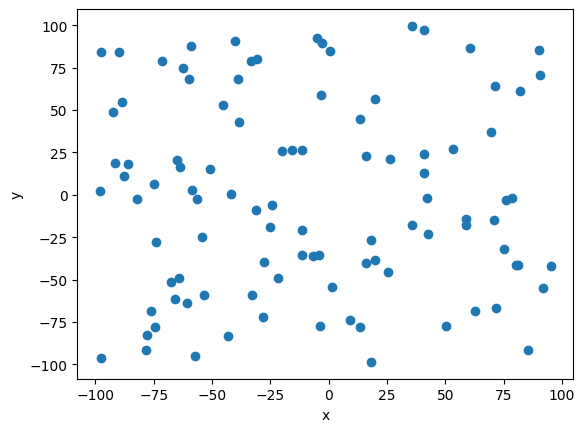
\includegraphics[width=\linewidth]{images/A.png}
        \caption{zbiór A}
    \end{subfigure}
    \begin{subfigure}{0.4\linewidth}
        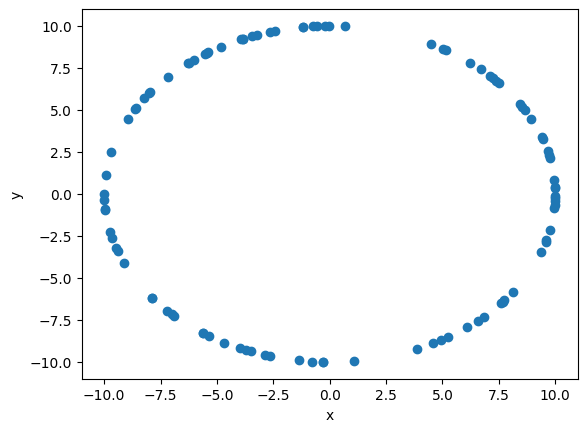
\includegraphics[width=\linewidth]{images/B.png}
        \caption{zbiór B}
    \end{subfigure}

    \begin{subfigure}{0.4\linewidth}
        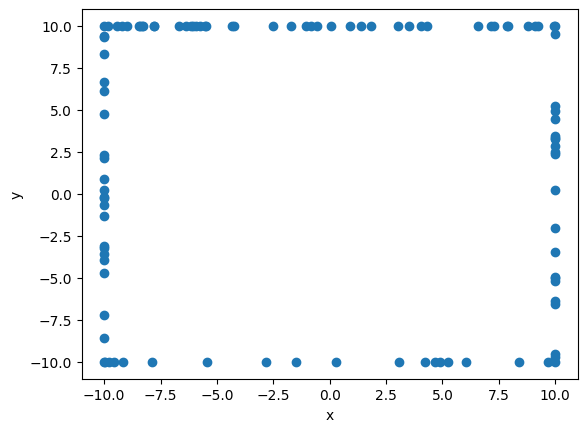
\includegraphics[width=\linewidth]{images/C.png}
        \caption{zbiór C}
    \end{subfigure}
    \begin{subfigure}{0.4\linewidth}
        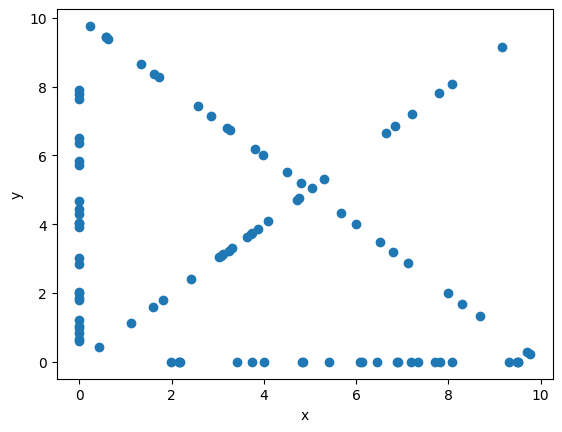
\includegraphics[width=\linewidth]{images/D.png}
        \caption{zbiór D}
    \end{subfigure}
    \caption{zbiory testowe}
\end{figure}

\section{Wyniki}
\subsection{wizualizacja}
Legenda:
\begin{itemize}
    \item \textcolor{blue}{Na niebiesko} oznaczono punkty ze zbioru
    \item \textcolor{black}{Na czarno} oznaczono otoczkę wypukłą oraz punkty w jej wierzchołkach
\end{itemize}

\begin{figure}[h]
    \centering
    \begin{subfigure}{0.4\linewidth}
        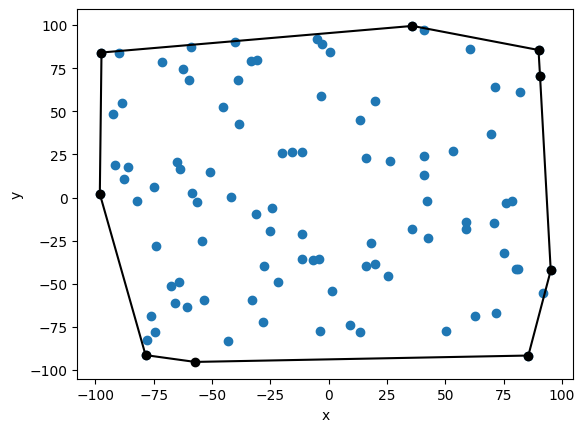
\includegraphics[width=\linewidth]{images/graham_a.png}
        \caption{algorytm Grahama}        
    \end{subfigure}
    \begin{subfigure}{0.4\linewidth}
        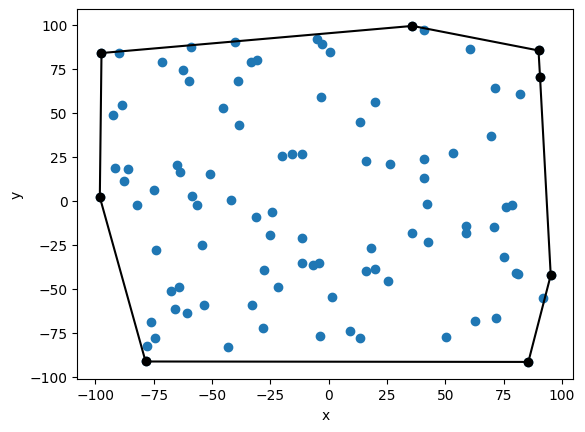
\includegraphics[width=\linewidth]{images/jarvis_a.png}
        \caption{algorytm Jarvisa}
    \end{subfigure}
    \caption{Zbiór A}
\end{figure}


\begin{figure}[H]
    \centering
    \begin{subfigure}{0.4\linewidth}
        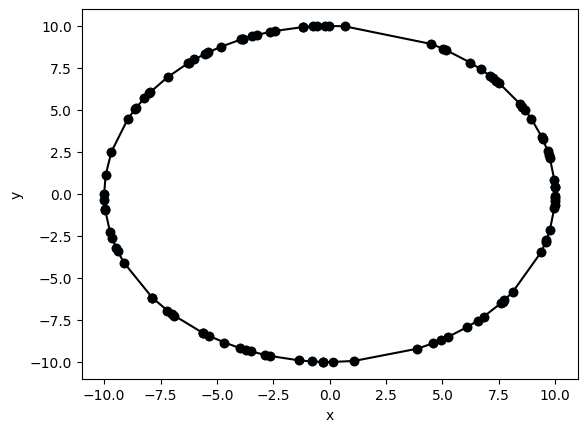
\includegraphics[width=\linewidth]{images/graham_b.png}
        \caption{algorytm Grahama}
    \end{subfigure}
    \begin{subfigure}{0.4\linewidth}
        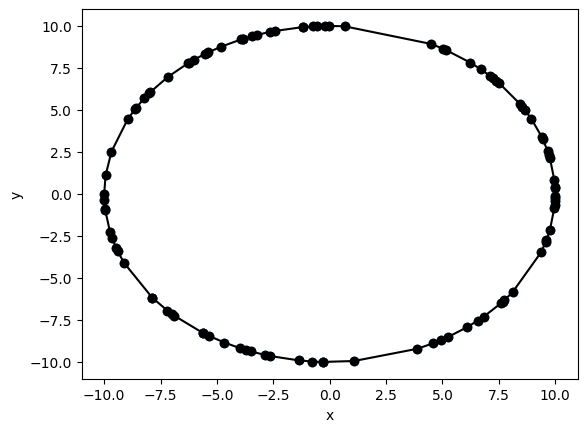
\includegraphics[width=\linewidth]{images/jarvis_b.png}
        \caption{algorytmy Jarvisa}
    \end{subfigure}
    \caption{zbiór B}
\end{figure}

\begin{figure}[H]
    \centering
    \begin{subfigure}{0.4\linewidth}
        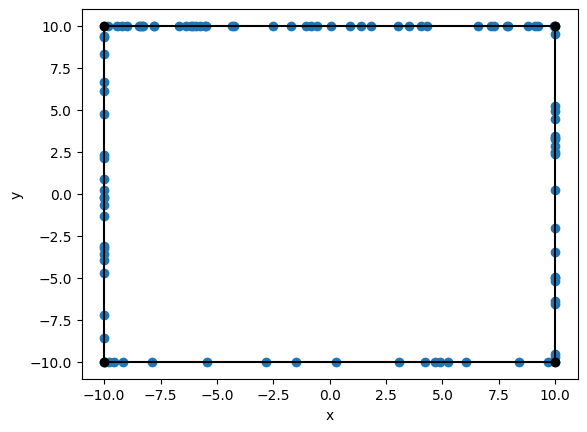
\includegraphics[width=\linewidth]{images/graham_c.png}
        \caption{algorytm Grahama}
    \end{subfigure}
    \begin{subfigure}{0.4\linewidth}
        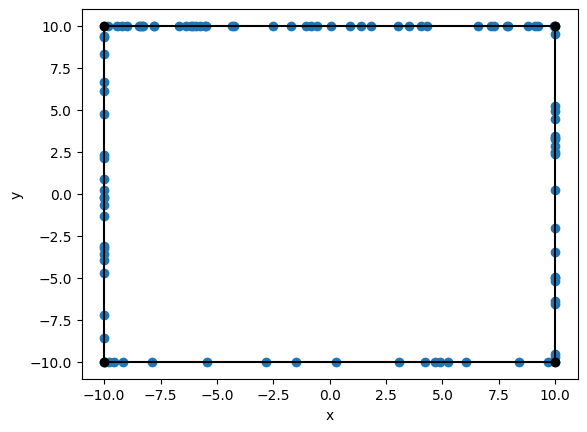
\includegraphics[width=\linewidth]{images/jarvis_c.png}
        \caption{algorytm Jarvisa}
    \end{subfigure}
    \caption{Zbiór C}
\end{figure}

\begin{figure}[H]
    \centering
    \begin{subfigure}{0.4\linewidth}
        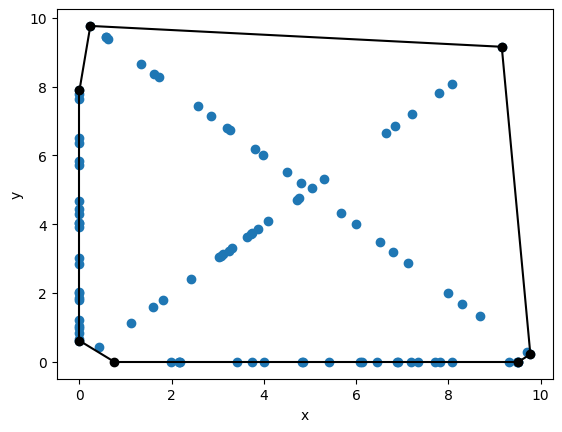
\includegraphics[width=\linewidth]{images/graham_d.png}
        \caption{algorytm Grahama}
    \end{subfigure}
    \begin{subfigure}{0.4\linewidth}
        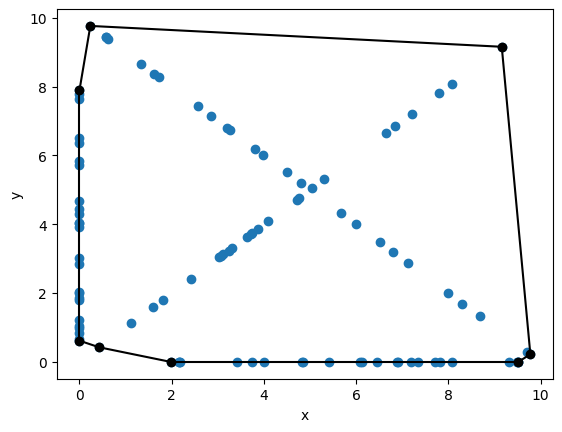
\includegraphics[width=\linewidth]{images/jarvis_d.png}
        \caption{algorytm Jarvisa}
    \end{subfigure}
    \caption{Zbiór D}
\end{figure}

Jak widać oba algorytmy poprawnie obliczyły i zwizualizowały otoczkę wypukłą dla prostych przykładów. Możemy założyć, że implementacja
jest poprawna. Gify pokazujące działanie algorytmu krok po kroku pozwolą lepiej zroozumiec działanie algorytmów.

\subsection{Test wydajności}
W tej sekcji porównamy jak zmienia się działanie algorytmów w każdym ze zbiorów na większym zakresie, większą liczbą punktów
oraz z różnymi wartościami dla epsilon. W komórkach tabel dane będą podane w postaci \textit{liczba wierzchołków w otoczce}/\textit{
czas pracy algorytmu w sekundach}. W tych testach:
\begin{itemize}
    \item \textbf{Zbiór A} - zbiór równomiernie rozłożonych punktów w przedziale $((-1000,-1000),(1000,1000))$
    \item \textbf{Zbiór B} - zbiór punktów położonych na okręgu o środku $(0,0)$ oraz promieniu $R=1000$
    \item \textbf{Zbiór C} - zbiór punktów położonych na krawędziach kwadratu o lewym dolnym wierzchołku $(-1000,-1000)$ i długości boku $l = 2000$
    \item \textbf{Zbiór D} - zbiór punktów położonych na przekątnych oraz dwóch krawędziach kwadratu o lewym dolnym
     wierzchołku $(-1000,-1000)$ i długości boku $l = 2000$
\end{itemize}

\subsubsection{$\epsilon=10^{-8}$}
\begin{table}[h]
    \centering
    \begin{tabular}{|c||c|c|c|c|}
        \hline
        liczba punktów & A & B & C & D \\
        \hline\hline
        1000 & 16/0.0027 & 1000/0.0019 & 4/0.0057 & 5/0.0021\\
        \hline
        2000 & 15/0.0056 & 1999/0.0041 & 4/0.0069 & 5/0.0047\\
        \hline
        5000 & 23/0.0157 & 4992/0.0118 & 4/0.0191 & 5/0.0128\\
        \hline
        10000 & 24/0.0319 & 9950/0.0265 & 4/0.0191 & 6/0.281\\
        \hline
        20000 & 28/0.0567 & 19713/0.0541 & 4/0.1841 & 7/0.0603\\
        \hline
        50000 & 33/0.1550 & 46914/0.1460 & 4/0.2420 & 6/0.1671\\
        \hline
        75000 & 32/0.4216 & 66755/0.2274 & 4/0.4998 & 7/0.3612\\
        \hline 
    \end{tabular}
    \caption{Tabela przedstawia wyniki dla algorytmu Grahama}
    \label{Graham_normalny}
\end{table}

\begin{table}[h]
    \centering
    \begin{tabular}{|c||c|c|c|c|}
        \hline
        liczba punktów & A & B & C & D \\
        \hline\hline
        1000 & 16/0.0030 & 999/0.0760 & 5/0.0014 & 5/0.0010\\
        \hline
        2000 & 14/0.0054 & 1998/0.2944 & 5/0.0027 & 5/0.0021\\
        \hline
        5000 & 26/0.0241 & 4991/1.9164 & 5/0.0067 & 6/0.0060\\
        \hline
        10000 & 23/0.0350 & 9950/7.5762 & 5/0.0134 & 6/0.0120\\
        \hline
        20000 & 29/0.0908 & 19713/31.2333 & 5/0.0280 & 7/0.0282\\
        \hline
        50000 & 33/0.2561 & 46721/197.7571 & 5/0.0686 & 6/0.0617\\
        \hline
        75000 & 32/0.4966 & 66562/434.8073 & 5/0.1358 & 7/0.1030\\
        \hline 
    \end{tabular}
    \caption{Tabela przedstawia wyniki dla algorytmu Jarvisa}
    \label{Jarvis_normalny}
\end{table}
\clearpage
\subsubsection{$\epsilon = 10^{-12}$}
\begin{table}[h]
    \centering
    \begin{tabular}{|c||c|c|c|c|}
        \hline
        liczba punktów & A & B & C & D \\
        \hline\hline
        1000 & 16/0.0027 & 999/0.0018 & 13/0.0057 & 8/0.0020\\
        \hline
        2000 & 14/0.0055 & 1999/0.0042 & 11/0.0055 & 5/0.0042\\
        \hline
        5000 & 26/0.0153 & 4999/0.0117 & 11/0.0145 & 7/0.0112\\
        \hline
        10000 & 23/0.0341 & 9996/0.0252 & 17/0.0335 & 6/0.294\\
        \hline
        20000 & 29/0.0567 & 19993/0.1535 & 11/0.0669 & 17/0.0511\\
        \hline
        50000 & 33/0.1562 & 49893/0.1488 & 7/0.1785 & 15/0.2480\\
        \hline
        75000 & 32/0.3204 & 74687/0.3476 & 10/0.3937 & 10/0.2212\\
        \hline 
    \end{tabular}
    \caption{Tabela przedstawia wyniki dla algorytmu Grahama}
    \label{Graham_zepsuty}
\end{table}

\begin{table}[h]
    \centering
    \begin{tabular}{|c||c|c|c|c|}
        \hline
        liczba punktów & A & B & C & D \\
        \hline\hline
        1000 & 16/0.0030 & 993/0.0714 & 12/0.0026 & 7/0.0014\\
        \hline
        2000 & 13/0.0050 & 1998/0.2919 & 433/0.1632 & 10/0.0038\\
        \hline
        5000 & 25/0.0243 & 4998/1.8652 & 1111/1.0538 & 45/0.0413\\
        \hline
        10000 & 22/0.0366 & 9994/7.5404 & 83/0.1834 & 4966/6.8453\\
        \hline
        20000 & 27/0.0845 & 19990/31.2117 & 1910/7.8585 & 11364/30.8067\\
        \hline
        50000 & 33/0.2547 & 49893/200.1075 & 31815/237.9071 & 134/1.2844\\
        \hline
        75000 & 32/0.4941 & 74674/441.9657 & 4726/99.9642 & 10623/137.9801\\
        \hline 
    \end{tabular}
    \caption{Tabela przedstawia wyniki dla algorytmu Jarvisa}
    \label{Jarvis_zepsuty}
\end{table}

\section{Analiza Wyników}
\subsection{Porównanie Działania Algorytmów}
\paragraph{Algorytm Grahama} - wykazał się dużą stabilnością i szybkością we wszystkich przypadkach testowych (tabela \ref{Graham_normalny}). Złożoność $O(nlogn)$
zdominowana przez etap sortowania kątowego, sprawia, że jest on przewidywalnie wydajny niezależnie od kształtu otoczki. Jest to
algorytm wydajny w ogólnym przypadku, który dobrze się sprawdza kiedy nie możemy poczynić założeń na temat zbioru punktów.

\paragraph{Algorytm Jarvisa} - pomimo kiepskiej złożoności w przypadku pesymistycznym $O(n^{2})$, algorytm był znacznie szybszy
w przypadku zbiorów C i D (tabela \ref{Jarvis_normalny}), w których niewiele punktów trafiało do otoczki wypukłej. W zbiorze A, pomimo że algorytm Jarvisa był
wolniejszy od algorytmu Grahama, to wciąż spisywał się nieźle. Problemem natomiast był zbiór B, który jest przypadkiem pesymistycznym
i w którym czas obliczeń rozciągał się do kilku minut. Ten algorytm warto implementować jedynie, jeżeli możemy zagwarantować
jego złożoność zbliżoną do liniowej.

\subsection{Porównanie Wartości $\epsilon$} 
Jak widać w tabeli \ref{Graham_zepsuty} i \ref{Jarvis_zepsuty}, wartość $\epsilon=10^{-12}$
zaburza działanie algorytmu dla zbiorów C, D. W zbiorze C oczekiwano jedynie 4 wierzchołków otoczki, natomiast w zbiorze D otoczka nie
powinna zawierać więcej niż 8 punktów. Wartość epsilon była na tyle mała, że algorytmy miały problem z poprawnym rozpoznaniem wierzchołków
współliniowych. W przypadku zbioru A, gdzie szansa na to, że 3 punkty będą współliniowe jest znikoma, nie stanowiło to problemu,
natomiast w zbiorze B, gdzie mamy gwarancję, że żadne 3 punkty nie są współliniowe znacząco poprawiło to wyniki w porównaniu do
$\epsilon=10^{-8}$ (tabele \ref{Graham_normalny} i \ref{Jarvis_normalny}). Nie zaoobserwowano znaczącego bezpośredniego wpływu wartości
$\epsilon$ na szybkość wykonania algorytmu. Algorytm Jarvisa został spowolniony jedynie przez wydłużenie otoczki przez błędy obliczeń
zmiennoprzecinkowych.

\section{Środowisko}
\begin{itemize}
    \item System operacyjny: Linux 6.17.9-arch1-1
    \item Procesor: AMD Ryzen 9800x3d
    \item Język programowania + translator: Python 3.13.7
    \item Środowisko: JupyterNotebook
    \item wynik !jupyter --version
        \begin{itemize}
        \item IPython          : 9.7.0
        \item ipykernel        : 7.1.0
        \item ipywidgets       : not installed
        \item jupyter\_client   : 8.6.3
        \item jupyter\_core     : 5.9.1
        \item jupyter\_server   : 2.17.0
        \item jupyterlab       : 4.5.0
        \item nbclient         : 0.10.2
        \item nbconvert        : 7.16.6
        \item nbformat         : 5.10.4
        \item notebook         : 7.5.0
        \item qtconsole        : not installed
        \item traitlets        : 5.14.3
    \end{itemize}
\end{itemize}
\end{document}